\chapter{\color{Millum}\textbf{Utfordringer}}
\newthought {Alle utviklingsprosjekter byr på utfordringer.} I dette kapittelet skal vi dykke litt dypere i de tekniske og menneskelige utfordringene vi hadde underveis i prosjeket.

\section{\textbf{Tekniske utfordringer}}

\subsubsection{\textbf{Håndtering av desimaltall}}

Millum sine kunder er stort sett basert i Skandinavia og vi har derfor vært nødt til å støtte flere språk i applikasjonen vår. I Norge og flere andre land brukes komma som desimalskille, mens andre land bruker for eksempel punktum ved håndtering av desimaltall. Når det gjelder håndtering av desimaltall har vi støtt på en utfordring som spiste mye mer arbeidstid enn forventet. 

Under en varetelling som vist tidligere \ref{fig:DesignInputStepper} gir vi bruker mulighet til å telle en vare med et inntastingsfelt \textit{eller} ved å trykke på pluss eller minus.

Et eksempel på å legge inn et inntastingsfelt med HTML
\begin{lstlisting}
<input type="number">
\end{lstlisting}

Standarden til Typescript når man har et inputfelt med tallverdier er at desimalskillet er punktum, og ikke godtar komma. Vi måtte derfor bruke inputfelt med tekstverdier for å tillate dette. Dette skapte videre problemer fordi ugyldige verdier som bokstaver, tegn og lignende kan bli fylt inn. Det er \textit{kun} tall som er gjeldende for inntastningsfeltet og for at det skal bli håndert riktig av applikasjonen må vi sørge for at bruker ikke skriver inn ugyldige tegn. I tillegg  vil det numeriske tastaturet på mobilen ikke vises på grunn av input-typen ``tekst``. 

Vi kom derfor frem til denne fremgangsmåten for å løse problemene

\begin{enumerate}
    \item \textbf{Fjerne ugyldige verdier.} Herunder alle bokstaver, spesialtegn, overflødige nuller og duplikater av skilletegn ved bruk av regulære utrykk og konvertere fra tekst til tall.
    
    \begin{figure}[H] 
        \centering
        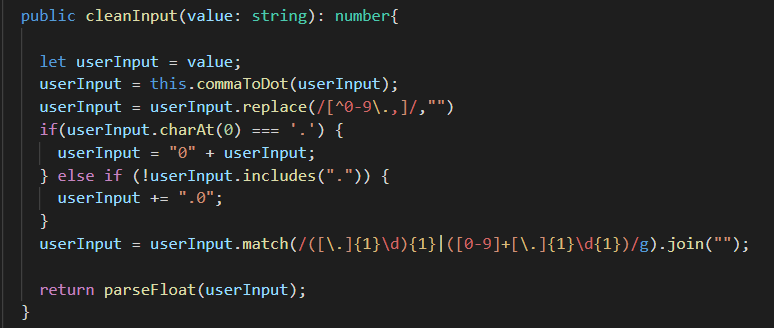
\includegraphics[width=120mm]{figures/Utfordringer/cleanInput.PNG}
        \caption{Bruk av regulære utrykk for å fjerne ugyldige verdier.}
    \end{figure}
    
    \item \textbf{Konvertere skilletegn} basert på brukerens språk ved å hente opp valgt språk, og sjekke hvilken standard for desimaltegn blir brukt.
    
    \begin{figure}[H] 
        \centering
        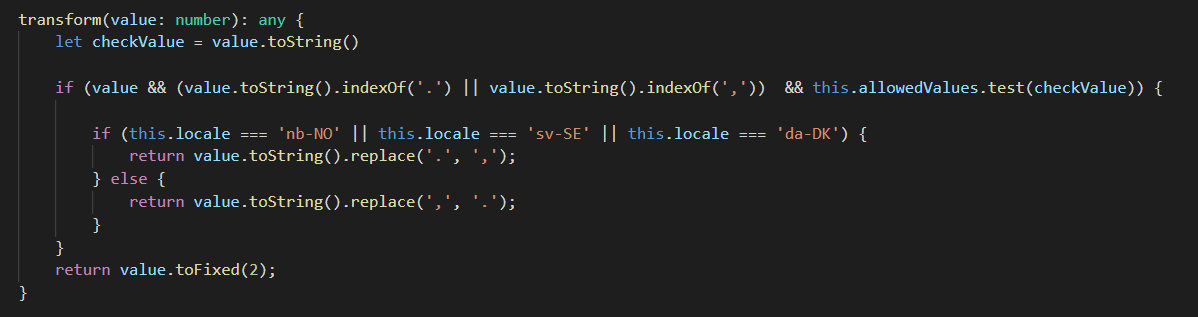
\includegraphics[width=120mm]{figures/Utfordringer/numericFormat.PNG}
        \caption{Kodesnutt av numericFormat-pipe.}
    \end{figure}
    
    \item \textbf{Tvinge keyboard til å kun vise tall} ved å sette input-modus til ''numeric''.
    
    \begin{figure}[H] 
        \centering
        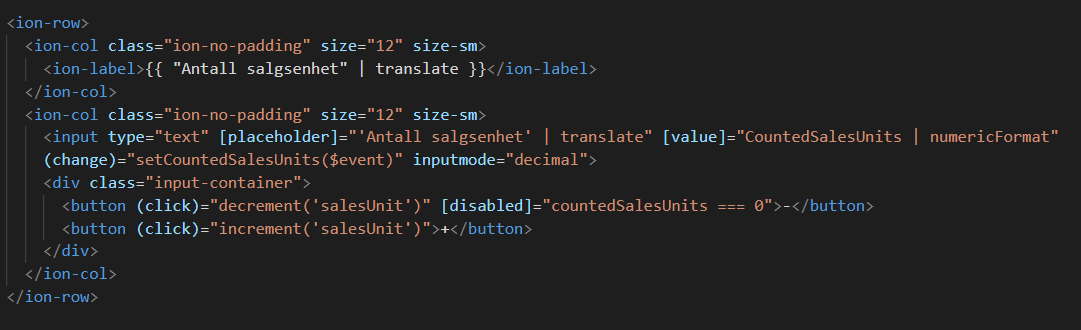
\includegraphics[width=120mm]{figures/Utfordringer/stock-taking-count-codeSnippet.PNG}
        \caption{Kodesnutt av et inntastningsfelt under en varetelling.}
    \end{figure}
    
\end{enumerate}


Med de tre punktene ovenfor har vi klart å eliminere hovedutfordringen ved å fremvise desimaltall etter hvilket språk som er i bruk. Dette var en ''task'' vi opprinnelig hadde satt av én arbeidsdag på å gjennomføre, men ettersom dette var en utfordring ingen av oss hadde støtt på tidligere gikk det nærmere tre arbeidsdager med diskusjon og testing. Enderesultatet oppfyller atferden inntastingsfeltene bør og må ha. I tillegg fikk vi  virkelig oppleve det å feilestimere tid under en ''task'' i Scrum-rammeverket. 


\section{\textbf{Andre utfordinger}}

I sammenheng med virusutbruddet av Covid-19 gikk oppdragsgiver den 19. Mars ut med permitteringsvarsler for samtlige ansatte i organisasjonen. Avdelingslederen var rask på banen til å følge opp oss for å sørge for at vi fortsatt kunne gjennomføre hovedoppgaven vår i så høy grad det var mulig. Dessverre hadde dette uventede konsekvenser for oss. Vi hadde blant annet ikke lenger mulighet til å gjennomføre planlagte brukertester med kunder, og vi ble nødt til å skrinlegge noe planlagt funksjonalitet. Siden utviklingsmiljøet til oppdragsgiveren var lukket var vi nødt til å få på plass VPN (Virtual Private Network. Brukes til å koble seg på lukket nett utenifra). Dessverre var det ikke mulig å koble seg på VPN på mobiltelefon som ga oss utfordringer med å jobbe hjemmefra. Til tross for dette hadde vi allerede kommet langt på løsningen og var tilpasningsdyktige i denne turbulente tiden. Det er i slike situasjoner man reflekterer over hvor viktig en god prosess er, så man alltid har mulighet til å tilpasse seg nye situasjoner.

Som en følge av permitteringssituasjonen hos oppdragsgiver hadde vi heller ikke mulighet til å teste applikasjonen i produksjonsmiljøer, og vi måtte derfor definere leveransekravet på nytt ettersom vi ikke kan lansere en applikasjon som ikke er testet med reel data. Selv om dette ikke var problematisk for vår del skulle vi gjerne ha fulgt hele løpet fra innsiktfasen til produksjonssetting som vi opprinnelig hadde planlagt. Vi kommer tilbake til vurdering av situasjonen i kapittel 9 (LINK HER)

